\section{Use Cases}
\label{sec:use-cases}

We design a representative use case that reflects workload heterogeneity, resource contention, and energy cost interactions across quantum and classical subsystems. 

We generate a synthetic workload consisting of 1,200 independent quantum circuit synthesis jobs, stored in a CSV file and submitted to the simulator as an external job trace. 

\begin{table}[t]
\centering
\caption{HybridCloudSim Use Case Configurations and Workload Parameters}
\label{tab:use-case-summary}
\begin{tabular}{p{0.31\linewidth} p{0.60\linewidth}}
\hline
\textbf{Category} & \textbf{Configuration} \\
\hline
Workload size & 1,200 hybrid synthesis jobs (CSV trace) \\

Quantum workload parameters &
\begin{tabular}[t]{@{}l@{}}
Number of qubits: 10 to 25 \\
Circuit depth: 37 to 99 \\
Shots per job: 1,000 to 5,000 \\
Iterations per job: 4 to 9 \\
Arrival process: Exponential ($\lambda \approx 0.36$)
\end{tabular} \\

Classical workload parameters &
\begin{tabular}[t]{@{}l@{}}
CPU units: 4 to 7 (qubit scaled) \\
Memory BW units: 4 to 7 (qubit scaled)
\end{tabular} \\

Quantum resources &
\begin{tabular}[t]{@{}l@{}}
2 $\times$ IBM Eagle r3 QPUs (127 qubits each) \\
IBM\_Quebec: 32,000 CLOPS \\
IBM\_Kyiv: 30,000 CLOPS
\end{tabular} \\

Classical resources &
\begin{tabular}[t]{@{}l@{}}
1 $\times$ CPU nodes \\
8 cores, 16 threads per node \\
Base / boost: 3.8 / 5.0 GHz \\
Memory bandwidth: 51.2 GB/s
\end{tabular} \\

Resource abstraction &
\begin{tabular}[t]{@{}l@{}}
CPU capacity = threads $\times$ cpu units \\
Mem BW capacity = GB/s $\times$ mem units
\end{tabular} \\

Energy pricing & \$0.18 per kWh \\

QPU power model &
\begin{tabular}[t]{@{}l@{}}
Static power draw: 50 kW each\\
\end{tabular} \\

CPU power model &
\begin{tabular}[t]{@{}l@{}}
Per job billing: constant at peak \\
CPU peak: 5.0 kW \\
Fleet power: affine, idle 30\% of peak
\end{tabular} \\

\hline
\end{tabular}
\end{table}

Table~\ref{tab:use-case-summary} summarizes the characteristics of the workload, infrastructure, and cost configuration used in our hybrid quantum classical cloud simulation. This consolidated view is intended to improve reproducibility and provide readers with a concise overview of the experimental setup. Here, \textit{cpu units} and \textit{memory units} represent normalized per thread compute capacity and per GB/s bandwidth capacity, respectively. The trace's classical columns are recorded but not consulted by the dispatcher: as in Section~\ref{sec:iter-setup}, every CPU phase is admitted against a fixed budget of 8 CPU and 20 memory bandwidth units.

We assume a fixed electricity price of \$0.18 per kWh, representative of commercial cloud pricing. Quantum devices are modeled with static power draw values to reflect the high baseline energy cost of superconducting systems, with each QPU assigned a power draw of 50 kW. These values are selected within the reported power consumption range of superconducting quantum computing systems~\cite{ezratty2021}.

A classical CPU node is assigned a device specific power envelope of 5.0\,kW, at which each job is billed for the duration of its own computation, while the node's instantaneous draw in the fleet view follows an affine model between an idle floor of 30\% of that envelope and the envelope itself. We note that absolute CPU power values are less critical in our study, as our results are driven by the relative energy imbalance between QPU and classical resources. The detailed models are provided in Section~\ref{sec:models}.

\subsection{Performance Evaluation}
\label{sec:performance-evaluation}

In this section, we evaluate the performance characteristics of the HybridCloudSim environment setup and analyze aggregate cloud resource usage to understand overall system behavior, followed by a time series analysis to capture temporal utilization dynamics.

In terms of cost, the mean energy cost per job is \$0.099556 $\pm$ 0.049350, with a median cost of \$0.0939 and a 95th percentile cost of \$0.190520, reflecting the right skewed cost distribution. Energy fraction statistics further confirm the dominant role of quantum execution, with a mean QPU energy fraction of 0.981943 $\pm$ 0.079422 and a mean CPU energy fraction of 0.018050 $\pm$ 0.079423. These results quantitatively reinforce the earlier observation that overall energy consumption and cost in hybrid quantum classical workloads are overwhelmingly driven by QPU operation, while classical resources contribute smaller but non negligible overheads.

\subsection{Time Series Resource Utilization}
\label{subsec:time-series-utilization}

\begin{figure}[t]
    \centering
    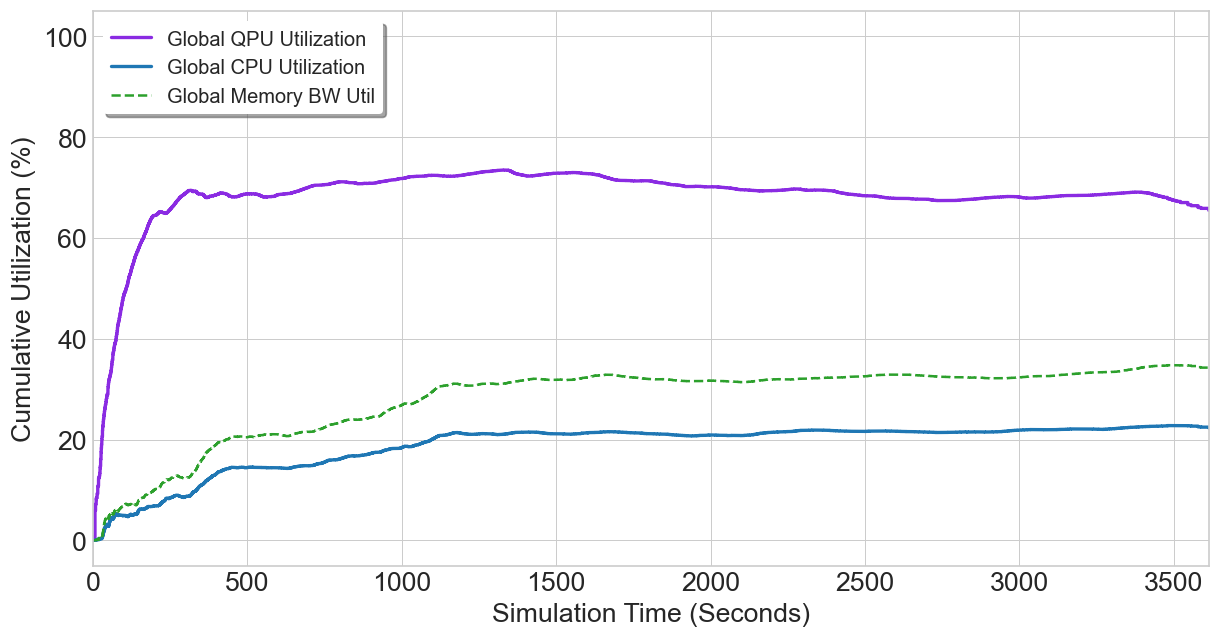
\includegraphics[width=0.99\linewidth]{Images/Performance/Cloud-utilization.png}
    \caption{Cumulative Cloud Resource Utilization Over Time.}
    \label{fig:cumulative_utilization}
\end{figure}

Figure~\ref{fig:cumulative_utilization} illustrates the cumulative time integrated resource utilization across the hybrid quantum cloud environment over a 3,764 second execution window. During the initial warm up phase ($t < 500\,\text{s}$), all three subsystem resources experience a steep ramp up in utilization as arriving workloads fill the system pipelines. The global quantum processing unit (QPU) utilization rises rapidly, stabilizing into a steady state regime between $67\%$ and $73\%$ between $t = 500\,\text{s}$ and $t = 3,500\,\text{s}$. This sustained high demand highlights the QPU as the primary performance bottleneck within the hybrid infrastructure. In contrast, classical resource demands stabilize at lower levels, with memory bandwidth cumulative utilization settling between $30\%$ and $35\%$ after $t \approx 1{,}200\,\text{s}$ and global CPU utilization settling near $20\%$ to $23\%$. The pronounced gap between QPU and CPU or memory utilization reflects the asymmetric nature of quantum classical workflows, where classical hardware spends significant time idle while waiting for long duration quantum circuit executions to complete. The detailed calculations are provided in Section~\ref{sec:instant_vs_cumulative}.

\subsection{Energy Consumption and Cost Analysis}
\label{subsec:energy-analysis}

We next analyze the energy characteristics of the hybrid quantum classical cloud environment. 

\subsubsection{Distribution of Energy Cost Across Jobs}

\begin{figure}[t]
    \centering
    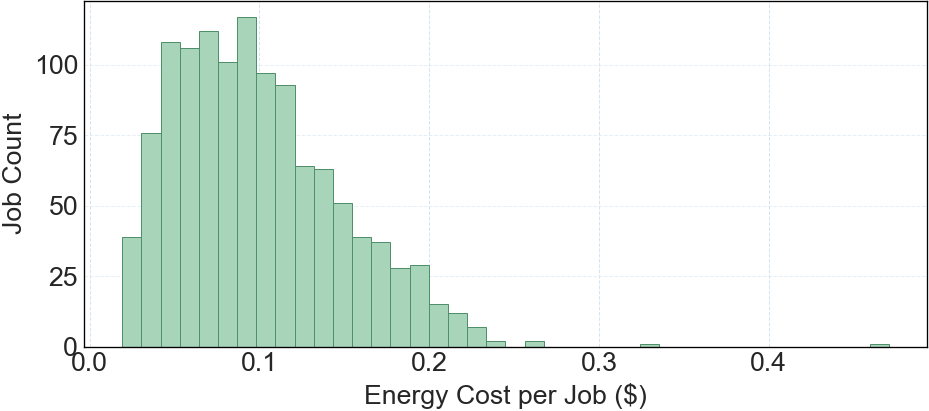
\includegraphics[width=0.99\linewidth]{Images/Performance/Energy-cost-distribution.png}
    \caption{Distribution of energy cost per job (\$) across executed workloads, showing a right-skewed distribution where the majority of jobs incur costs under \$0.20, with a small tail extending up to \$0.48.}
    \label{fig:energy-cost-distribution}
\end{figure}

Figure~\ref{fig:energy-cost-distribution} shows the distribution of energy cost per job, computed using the modeled energy consumption and a fixed electricity price. The distribution is right skewed, with most jobs clustered at lower costs and a diminishing number of higher cost outliers.

This behavior arises from variability in circuit depth, qubit count, execution duration, and iterative workload structure. Importantly, the absence of multimodal behavior suggests that cost variation is driven by continuous workload heterogeneity rather than discrete execution regimes. 

\subsubsection{Time Series Power Consumption}

\begin{figure}[t]
    \centering
    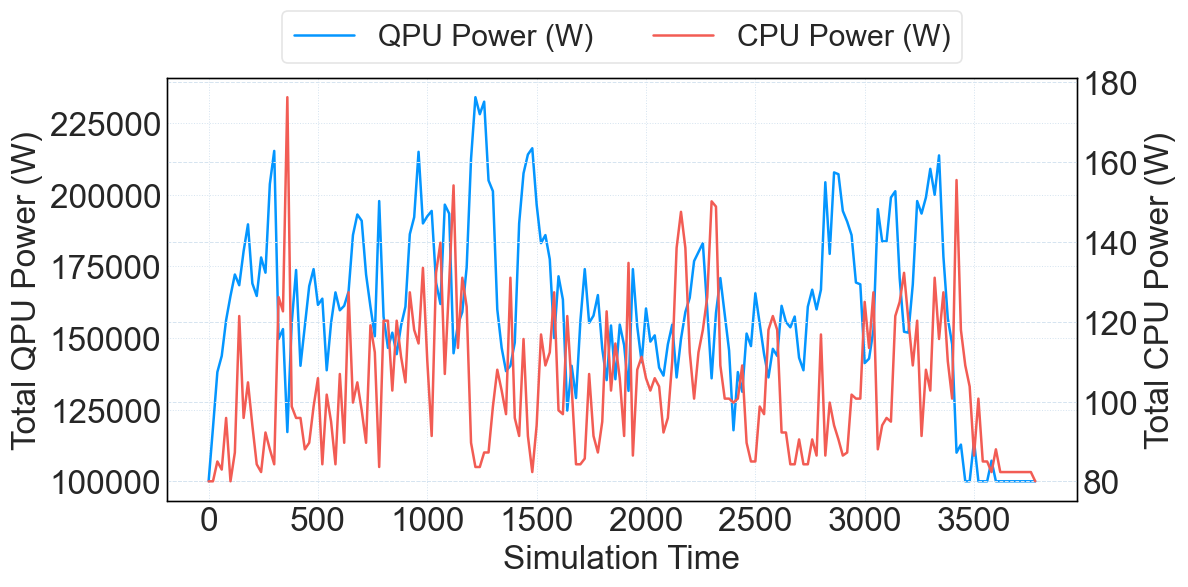
\includegraphics[width=0.99\linewidth]{Images/Performance/Power-timeseries.png}
    \caption{Time-series profile of QPU (left y-axis, blue) and CPU (right y-axis, red) power consumption in Watts over total simulation time (seconds) under the load dependent power variant described in the text, illustrating the dynamic resource utilization and power fluctuations during hybrid quantum-classical execution.}
    \label{fig:power-timeseries}
\end{figure}

Figure~\ref{fig:power-timeseries} illustrates the time series power consumption of QPU and CPU resources. It is drawn from the job records by an illustrative load dependent variant of the power model rather than by Eq.~\eqref{eq:power}: the two QPUs draw their combined 100~kW baseline rising linearly toward 300~kW with the fraction of a fixed 640 qubit reference capacity claimed by admitted jobs, each counted from admission to release, and the CPU node draws 80~W rising toward 360~W with the 1.3 power of its unit utilization. Because admitted jobs are counted before a connected region is secured, the claimed fraction measures demand pressure on the fleet rather than physical qubit occupancy, and under contention it exceeds what 254 qubits could hold. The QPU power remains persistently high, fluctuating within a range of approximately 100{,}000 to 235{,}000~W around its baseline operating level. These variations coincide with active execution periods, but they sit on top of a fixed 100~kW cryogenic cooling and control baseline that the two QPUs draw even when idle, which alone accounts for over 60\% of the 160~kW mean draw.

In contrast, CPU power operates at a significantly lower scale on this variant's 80 to 360~W envelope, distinct from the 5.0~kW billing rate, varying between roughly 80 and 175~W over time. Unlike the QPU, CPU power exhibits more pronounced relative fluctuations that correlate with classical execution phases, job arrivals, and orchestration activities. This stark separation in power magnitude between QPU and CPU resources indicates that energy optimization in hybrid quantum classical environments is primarily driven by QPU utilization efficiency rather than classical compute scaling.

As shown in Fig.~\ref{fig:energy_usage}, the plotted series spans an aggregate QPU power draw of approximately 100 to 235~kW for a configuration consisting of two superconducting QPUs, corresponding to roughly 50 to 117~kW per QPU. We note that these results are contingent on the chosen configuration parameters, taking Ezratty et al.~\cite{ezratty2021} as the baseline reference. Modifying the system or workload inputs will naturally alter the simulation outcomes. This sensitivity is a key advantage of our highly configurable framework.
